\section{System Block Diagram}

\tikzset{
    block/.style = {
        rectangle, 
        rounded corners, 
        minimum width=3cm, 
        minimum height=1cm, 
        align=center, 
        draw=black, 
        fill=white
    },
    subblock/.style = {
        rectangle, 
        minimum width=1.5cm, 
        minimum height=0.7cm, 
        align=center, 
        draw=black, 
        fill=white
    },
    arrow/.style = {
        thick, 
        -{Stealth[scale=1.2]}
    }
}

\begin{tikzpicture}[node distance=1.2cm]

% UAV System
\node[block, minimum width=7cm, minimum height=3cm] (uav) {UAV};
    \node[subblock] (pi) at ([xshift=0cm, yshift=0cm]uav.north west) {RPi};
    \node[subblock] (camera) at ([xshift=0cm, yshift=0cm]uav.south west) {Camera};
    \node[subblock] (receiver) at ([xshift=0cm, yshift=-1.5cm]uav.north east) {Receiver\\Control};

% Ground System (to the left/west of UAV)
\node[block, right=4cm of uav] (ground) {Ground\\Transmitter};

% Image Upscaling just below Camera
\node[block, below=2cm of uav] (upscale) {Image Upscaling\\(Deep Learning)};

% Land Use Classification below Image Upscaling
\node[block, below=of upscale] (classify) {Land Use\\Classification};
\node[block, below=of classify] (analysis) {Result\\Analysis};

% Data Flow
\begin{scope}[arrow]
    \draw (ground.west) -- (receiver.east); % straight line
    \draw (uav.south) -- node[right, xshift=0.2cm] {Raw\\Images} (upscale.north);
    \draw (upscale) -- (classify);
    \draw (classify) -- (analysis);
\end{scope}

% Legend

\node[align=center] at ($(analysis.south) + (0,-1)$) 
    {\footnotesize \textbf{Figure~\thefigure: System Block Diagram of UAV System}};

\end{tikzpicture}
 
\subsection{System Description}

The system consists of a fixed-wing UAV platform equipped with essential components for flight and data collection. The UAV includes:

\begin{itemize}
    \item \textbf{ESC (Electronic Speed Controller):} Regulates the speed of the motor driving the propeller.
    \item \textbf{Propeller:} Provides thrust for UAV flight.
    \item \textbf{4 Servos:} Control the movement of aerodynamic surfaces like ailerons, elevator, and rudder for flight maneuverability.
    \item \textbf{UAV Receiver:} Receives control signals from the ground-based transmitter.
    \item \textbf{Raspberry Pi + Camera Module:} Captures aerial images during flight.
\end{itemize}

The ground transmitter sends flight control commands to the UAV receiver. The Raspberry Pi processes input from the onboard camera and stores captured images.

These images are then passed to the image upscaling module using deep learning methods, enhancing the resolution and clarity. The upscaled images are further processed through a classification model to identify land use categories.
Finally, the results from the classification are analyzed for insights, contributing to high-resolution land use mapping from UAV-acquired data.

\section{Flowchart}
\begin{figure}[H]
\centering
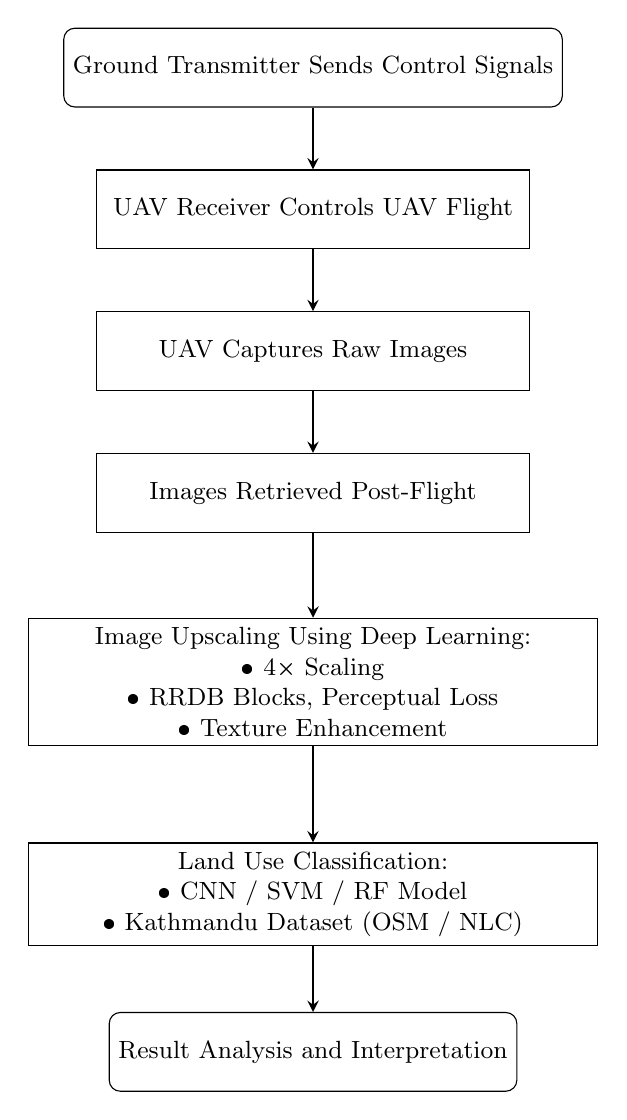
\begin{tikzpicture}[node distance=1.8cm, every node/.style={font=\small}] % increased node distance

\tikzstyle{startstop} = [rectangle, rounded corners, minimum width=3.5cm, minimum height=1cm, text centered, draw=black, fill=white]
\tikzstyle{process} = [rectangle, minimum width=5.5cm, minimum height=1cm, text centered, draw=black, fill=white]
\tikzstyle{arrow} = [thick,->,>=stealth]

\node (tx) [startstop] {Ground Transmitter Sends Control Signals};
\node (rx) [process, below of=tx] {UAV Receiver Controls UAV Flight};
\node (cam) [process, below of=rx] {UAV Captures Raw Images};
\node (ret) [process, below of=cam, yshift=-0cm] {Images Retrieved Post-Flight};
\node (upscale) [process, below of=ret, yshift=-0.6cm, text width=7cm] {
Image Upscaling Using Deep Learning:\\
• 4× Scaling\\
• RRDB Blocks, Perceptual Loss\\
• Texture Enhancement
};
\node (classify) [process, below of=upscale, yshift=-0.9cm, text width=7cm] {
Land Use Classification:\\
• CNN / SVM / RF Model\\
• Kathmandu Dataset (OSM / NLC)
};
\node (result) [startstop, below of=classify,yshift=-0.2cm] {Result Analysis and Interpretation};

% Arrows
\draw [arrow] (tx) -- (rx);
\draw [arrow] (rx) -- (cam);
\draw [arrow] (cam) -- (ret);
\draw [arrow] (ret) -- (upscale);
\draw [arrow] (upscale) -- (classify);
\draw [arrow] (classify) -- (result);

\end{tikzpicture}
\caption{Flowchart of the UAV-based Land Use Mapping Methodology}
\label{fig:flowchart}
\end{figure}

\section{Evaluation Plan}

The evaluation of the proposed UAV system will be carried out in three major phases, focusing on flight performance, data acquisition quality, and land use classification accuracy.

\subsection{Flight Performance Evaluation}
\begin{itemize}
    \item \textbf{Stability and Control:} The UAV's ability to respond to transmitter inputs will be tested under varying weather conditions. Metrics include roll, pitch, yaw response times, and return-to-home accuracy.
    \item \textbf{Endurance Testing:} Flight duration will be measured using a fully charged battery under standard payload conditions.
    \item \textbf{Component Reliability:} Each hardware component (ESC, servos, receiver, etc.) will be assessed for thermal stability and consistency across multiple flights.
\end{itemize}

\subsection{Image Data Quality Evaluation}
\begin{itemize}
    \item \textbf{Resolution Improvement:} The effectiveness of the deep learning-based upscaling model will be evaluated using PSNR (Peak Signal-to-Noise Ratio) and SSIM (Structural Similarity Index).
    \item \textbf{Dataset Diversity:} Images will be captured across diverse terrains (urban, agricultural, forested) to test generalizability.
    \item \textbf{Lighting and Clarity:} Assessment under different lighting conditions (morning, afternoon, dusk) to ensure usable imagery.
\end{itemize}

\subsection{Land Use Classification Evaluation}
\begin{itemize}
    \item \textbf{Accuracy Metrics:} Models (CNN, SVM, RF) will be evaluated using precision, recall, F1-score, and overall accuracy.
    \item \textbf{Confusion Matrix Analysis:} To identify class-wise performance and misclassifications.
    \item \textbf{Comparative Benchmarking:} Results will be compared against existing annotated datasets such as OpenStreetMap (OSM) and National Land Cover (NLC).
\end{itemize}

\subsection{System Integration Evaluation}
\begin{itemize}
    \item \textbf{End-to-End Pipeline Test:} A complete workflow test—from flight to image capture, upscaling, classification, and result analysis—will be conducted to validate system synchronization.
    \item \textbf{Latency Measurement:} Time taken from data acquisition to final analysis output will be recorded and optimized.
\end{itemize}

The outcomes from these evaluations will guide further optimization in both hardware setup and software processing pipelines, ensuring a robust and scalable UAV-based land mapping system.

